\chapter{Non-parametric methods}

\section{Intro}

Neural networks have adaptable complexity, in the sense that we can
try different structural models and use cross validation to find one
that works well on our data.  Beyond neural networks, we may further
broaden the class of models that we can fit to our data, for example
as illustrated by the techniques introduced in this chapter.

Here, we turn to models that automatically adapt their complexity to
the training data.  The name {\em non-parametric methods} is
misleading: it is really a class of methods that does not have a fixed
parameterization in advance.  Some non-parametric models, such as
decision trees, which we might call {\em semi-parametric methods}, can
be seen as dynamically constructing something that ends up looking
like a more traditional parametric model, but where the actual
training data affects exactly what the form of the model will be.
Other non-parametric methods, such as nearest-neighbor, rely directly
on the data to make predictions and do not compute a model that
summarizes the data.

The semi-parametric methods tend to have the form of a composition of
simple models.  We'll look at:
\begin{itemize}
\item {\em Tree models}:  (section~\ref{sec:np_trees}) partition the input space and use
  different simple predictions on different regions of the space;
  this increases the hypothesis space.
\item {\em Additive models}:  (section~\ref{sec:np_bagging}) train several different classifiers
  on the whole space and average the answers;  this decreases 
  the estimation error.
\item{\em Nearest neighbor models}: (section~\ref{sec:np_nn}) don't
  process data at training time, but do all the work when making
  predictions, by looking for the closest training example to a given
  new data point.
\end{itemize}
{\em Boosting} is a way to construct an additive model that decreases
both estimation and structural error, but we won't
address it in this class.

Why are we studying these methods, in the heyday of neural networks?
\begin{itemize}
\item They are fast to implement and have few or no hyper-parameters
  to tune.
\item They often work as well or better than more complicated methods.
\item Both can be easier to explain to a human user:  decision-trees
  are fairly directly human-interpretable and nearest neighbor methods
  can justify their decision to some extent by showing a few training
  examples that the prediction was based on.
\end{itemize}
    
%%%%%%%%%%%%%%%%%%%%%%%%%%%%%%%%%%%%%%%%%%%%%%%%%%%%%%%%%%%%%%%%%%%%%%%%%%%%%
\section{Trees}
\label{sec:np_trees}

The idea here is that we would like to find a partition of the input
space and then fit very simple models to predict the output in each
piece.  The partition is described using a (typically binary)
``decision tree,''  which recursively splits the space.

These methods differ by:
\begin{itemize}
\item The class of possible ways to split the space at each node;
  these are generally linear splits, either aligned with the axes of
  the space, or sometimes more general classifiers.
\item The class of predictors within the partitions;  these are often
  simply constants, but may be more
  general classification or regression models.
\item The way in which we control the complexity of the hypothesis:
  it would be within the capacity of these methods to have a separate
  partition for each individual training example.
\item The algorithm for making the partitions and fitting the models.
\end{itemize}

The primary advantage of tree models is that they are easily interpretable
by humans.  This is important in application domains, such as
medicine, where there are human experts who often ultimately make 
critical decisions and who need to feel confident in their
understanding of recommendations made by an algorithm.

\begin{examplebox}{\bf Example:} 
Here is a sample decision tree (reproduced from Breiman, Friedman, Olshen, Stone (1984)):

\tikzstyle{vertex}=[draw,fill=black!15,rectangle,minimum size=20pt,inner sep=8pt]
\tikzstyle{leafgreen}=[draw,fill=green!15,rectangle,minimum size=20pt,inner sep=8pt]
\tikzstyle{leafred}=[draw,fill=red!15,rectangle,minimum size=20pt,inner sep=8pt]

\begin{center}
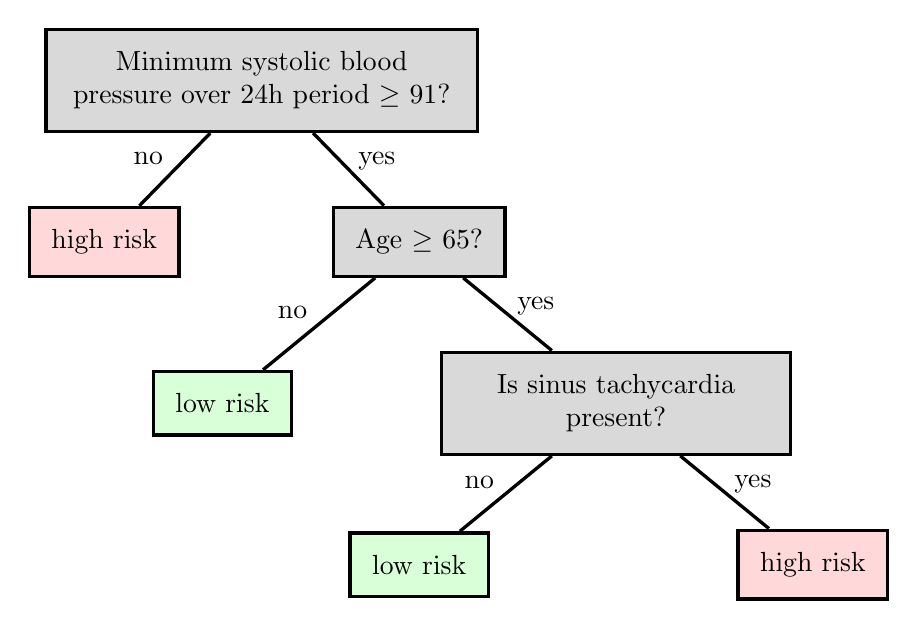
\begin{tikzpicture}[very thick,level distance=2.05cm,level 1/.style={sibling distance=40mm},level 2/.style={sibling distance=5cm}]
\node [vertex] (r){\begin{minipage}{14em}{\begin{center}Minimum systolic blood pressure over 24h period $\geq$ 91?\end{center}}\end{minipage}}
  child {
    node [leafred] (a) {high risk}
    edge from parent node[left,draw=none,xshift=-0.4pt,yshift=4pt] {no} 
  }
  child {
    node [vertex] {Age $\geq$ 65?}
    child {
      node [leafgreen] {low risk}
      edge from parent node[left,draw=none,xshift=-0.4pt,yshift=4pt] {no} 
    }
    child {
      node [vertex] {\begin{minipage}{11em}{\begin{center}Is sinus tachycardia present?\end{center}}\end{minipage}}
      child {node [leafgreen] {low risk}
        edge from parent node[left,draw=none,xshift=-0.4pt,yshift=4pt] {no} 
      }
      child {node [leafred] {high risk}
        edge from parent node[right,draw=none,xshift=-0.4pt,yshift=3pt] {yes} 
      }
      edge from parent node[right,draw=none,xshift=-0.4pt,yshift=3pt] {yes} 
    }
    edge from parent node[right,draw=none,xshift=-0.4pt,yshift=3pt] {yes} 
  };
\end{tikzpicture}
\end{center}


\end{examplebox}

These methods are most appropriate for domains where the input space
is not very high-dimensional and where the individual input features
have some substantially useful information individually or in small
groups.   They would not be good for image input, but might be good in
cases with, for example, a set of meaningful measurements of the
condition of a patient in the hospital.

We'll concentrate on the CART/ID3 family of algorithms, which were
invented independently in the statistics and the artificial
intelligence communities.  They work by greedily constructing a
partition, where the splits are {\em axis aligned} and by fitting a
{\em constant} model in the leaves.  The interesting questions are how
to select the splits and how to control complexity.  The regression
and classification versions are very similar.

\subsection{Regression}

\def\Rfeat{R}
\def\Rdata{\hat{R}}

The predictor is made up of
\begin{itemize}
\item a partition function, $\pi$, mapping elements of the input space into
  exactly one of $M$ regions, $\Rfeat_1, \ldots, \Rfeat_M$, and
\item a collection of $M$ output values, $O_m$, one for each region.
\end{itemize}

If we already knew a division of the space into regions, we would set
$O_m$, the constant output for region $\Rfeat_m$, to be the average of
the training output values in that region;  that is:
\[O_m = {\rm average}_{\{i \mid \ex{x}{i} \in R_m\}}\ex{y}{i}\;\;.\]
Define the error in a region as
\begin{equation}
  E_m = \sum_{\{i \mid \ex{x}{i} \in R_m\}}(\ex{y}{i} - O_m)^2\;\;.
\end{equation}
Ideally, we would select the partition to minimize
\begin{equation}
  \lambda M + \sum_{m=1}^M E_m\;\;,
\end{equation}
for some regularization constant $\lambda$.  It is enough to search over all
partitions of the training data (not all partitions of the input
space!) to optimize this, but the problem is NP-complete.
\question{Be sure you understand why it's enough to consider all
  partitions of the training data, if this is your objective.}

\subsubsection{Building a tree}
So, we'll be greedy.  We establish a criterion, given a set of data,
for finding the best single split of that data, and then apply it
recursively to partition the space.  We will select the partition of
the data that {\em minimizes the sum of the mean squared errors of
  each partition.}

Given a data set $D$, let 
\begin{itemize}
\item $\Rdata^+_{j,s}(D) = \{x \in D \mid x_j \geq s\}$ be the set of
  examples \note{A small subtlety: $\Rdata^+_{j,s}$ is a subset of data, but $\Rfeat_m$ is a partition of the feature space.}
in data set $D$ whose feature value in dimension $j$ is greater
  than or equal to split point $s$;
\item $\Rdata^-_{j,s}(D) = \{x \in D \mid x_j < s\}$ be the set of examples
  in $D$ whose feature value in dimension $j$ is less than $s$; 
\item $\hat{y}^+_{j,s} = {\rm average}_{\{i \mid \ex{x}{i} \in
    \Rdata^+_{j,s}(D)\}}\ex{y}{i} $ be the average $y$ value of the data
  points in set $\Rdata^+_{j,s}(D)$; and 
\item $\hat{y}^-_{j,s} = {\rm average}_{\{i \mid \ex{x}{i} \in
    \Rdata^-_{j,s}(D)\}}\ex{y}{i} $ be the average $y$ value of the data
  points in set $\Rdata^-_{j,s}(D)$.
\end{itemize}
Now, here is the pseudocode. \\

\noindent ${\bf BuildTree}(D,k)$:
\begin{itemize}
\item If $|D| \leq k$: return ${\rm Leaf}(D)$
\item Find the dimension $j$ and split point $s$ that minimizes:
      $E_{\Rdata^-_{j,s}(D)} + E_{\Rdata^+_{j,s}(D)}\;\;.$
\item Return ${\bf Node}(j, s, {\bf BuildTree}(\Rdata^-_{j,s}(D,k)), {\bf BuildTree}(\Rdata^+_{j,s}(D,k))$
\end{itemize}

Each call to {\bf BuildTree} considers $O(d n)$ splits (for $d$ dimensions, since we only need to
split between each data point in each dimension); each requires
$O(n)$ work where $n$ is the number of data points considered ($n = |D|$
if all data points in $D$ are used).
\question{Concretely, what would be a good set of split-points to
  consider for dimension $j$ of a dataset $D$?}

\subsubsection{Pruning}
It might be tempting to regularize by using a somewhat large
value of $k$, or by stopping when splitting a node does not significantly
decrease the error.  One problem with short-sighted stopping criteria
is that they might not see the value of a split that will require one
more split before it seems useful.
\question{Apply the decision-tree algorithm to the XOR problem in two
  dimensions.  What is the training-set error of all possible
  hypotheses based on a single split?}
So, we will tend to build a tree that is too large, and then prune it
back. 

Define {\em cost complexity} of a tree $T$, where $m$ ranges over its
leaves as 
\begin{equation}
C_\alpha(T) = \sum_{m = 1}^{|T|} E_m(T) + \alpha |T|\;\;.
\end{equation}

\noindent
and $|T|$ is the number of leaves.
For a fixed $\alpha$, we can find a $T$ that (approximately) minimizes
$C_\alpha(T)$ by ``weakest-link'' pruning:
\begin{itemize}
\item Create a sequence of trees by successively removing the
  bottom-level split that minimizes the increase in overall error,
  until the root is reached.
\item Return the $T$ in the sequence that minimizes the criterion.
\end{itemize}
We can choose an appropriate $\alpha$ using cross validation.

\subsection{Classification}

The strategy for building and pruning classification trees is very
similar to the strategy for regression trees.  

Given a region $\Rfeat_m$ corresponding to a leaf of the tree, we would
pick the output class $y$ to be the value that exists most frequently
(the {\em majority value}) in the data points whose $x$ values are in
that region:
\[O_m = {\rm majority}_{\{i \mid \ex{x}{i} \in \Rfeat_m\}}\ex{y}{i}\;\;.\]
Define the error in a region as the number of data points that do not
have the value $O_m$:
\[E_m = \left|\{i \mid \ex{x}{i} \in \Rfeat_m \;\text{and}\; \ex{y}{i} \not
  = O_m\}\right|\;\;.\]
Define the {\em empirical probability} of an item from class $k$
occurring in region $m$ as:
\[\hat{P}_{mk} = \hat{P}(\Rfeat_m)(k) = \frac{\left|\{i \mid \ex{x}{i} \in
    \Rfeat_m \;\text{and}\; \ex{y}{i} = k\}\right|}{N_m}\;\;,\]
where $N_m$ is the number of training points in region $m$.
We'll define the empirical probabilities of split values, as well,
for later use.
\[\hat{P}_{mjv} = \hat{P}(\Rfeat_{mj})(v) = \frac{\left|\{i \mid \ex{x}{i} \in
    \Rfeat_m \;\text{and}\; \ex{x}{i}_j \geq v\}\right|}{N_m}\]

\paragraph*{Splitting criteria}
In our greedy algorithm, we need a way to decide which split to make
next.  There are many criteria that express some measure of the 
``impurity'' in child nodes.  Some measures include:
\begin{itemize}
\item {\em Misclassification error}: 
  \begin{equation}
    Q_m(T) = \frac{E_m}{N_m} = 1 - \hat{P}_{mO_m}
    \end{equation}
\item {\em Gini index}:
  \begin{equation}
    Q_m(T) = \sum_k \hat{P}_{mk}(1 - \hat{P}_{mk})
    \end{equation}
\item {\em Entropy}: 
  \begin{equation}
    Q_m(T) = H(\Rfeat_m) = - \sum_k \hat{P}_{mk} \log_2 \hat{P}_{mk}
    \end{equation}
So that this is well-defined when $\hat{P} = 0$, we will stipulate that $0
\log_2 0 = 0$.
\end{itemize}
They are very similar, and it's not entirely obvious which one is
better.   We will focus on entropy, just to be concrete.

Analogous to how for regression we choose the dimension $j$ and split
$s$ that minimizes $E_{R_{j,v}^{+}(D)}+E_{R_{j,v}^{-}(D)}$, for
classification we choose the dimension $j$ and split $v$ that
minimizes the weighted entropy $$ \hat{P}_{mjv} H(R_{j,v}^{+}) +
(1-\hat{P}_{mjv}) H(R_{j,v}^{-}), $$ where note that $\hat{P}_{mjv}$
is the fraction of points with dimension $j$ in split $v$ occurring in region $m$ (one branch of the tree), 
and $1-\hat{P}_{mjv}$
is the complement (the other branch).
Choosing the split that minimizes the entropy of the children is
equivalent to maximizing the {\em information gain} of the test $X_j =
v$, defined by 
\begin{eqnarray}
{\rm infoGain}(X_j = v, \Rfeat_m) & = & H(\Rfeat_m) - 
\left(\hat{P}_{mjv}H(\Rdata^+_{j, v}) + (1 - \hat{P}_{mjv})H(\Rdata^-_{j, v})\right)
\end{eqnarray}

In the two-class case, all the criteria have the values
\[
\begin{cases}
0.0 & \text{when $\hat{P}_{m0} = 0.0$}\\
0.0 & \text{when $\hat{P}_{m0} = 1.0$}
\end{cases}
\]
The respective impurity curves are shown below, where $p = \hat{p
}_{m0}$:
\begin{center}
\includegraphics[scale=0.5]{figures/impurity.png}
\end{center}
There used to be endless haggling about which one to use.  It seems to
be traditional to use:
\begin{itemize}
\item Entropy to select which node to split while growing the tree
\item Misclassification error in the pruning criterion
\end{itemize}

\noindent
As a concrete example, consider the following images:
\begin{center}
\includegraphics[scale=1]{figures/dt_points.png}
\includegraphics[scale=1]{figures/dt_soln.png}
\end{center}
The left image depicts a set of labeled data points and the right shows a partition into regions by a decision tree.

\paragraph*{Points about trees}

There are many variations on this theme:
\begin{itemize}
\item Linear regression or other regression or classification
  method in each leaf
\item Non-axis-parallel splits: e.g., run a classification algorithm (with non-linear features) for a while to
  get a split.
\end{itemize}

\noindent What's good about trees:
\begin{itemize}
\item Easily interpretable
\item Fast to train!
\item Easy to handle multi-class classification
\item Easy to handle different loss functions (just change predictor
  in the leaves)
\end{itemize}
What's bad about trees:
\begin{itemize}
\item High estimation error:  small changes in the data can result in very big
  changes in the hypothesis.
\item Often not the best predictions
\end{itemize}

\paragraph*{Hierarchical mixture of experts}  Make a ``soft'' version
of trees, in which the splits are probabilistic (so every point has
some degree of membership in every leaf).  Can be trained with a form
of gradient descent.

%%%%%%%%%%%%%%%%%%%%%%%%%%%%%%%%%%%%%%%%%%%%%%%%%%%%%%%%%%%%%%%%%%%%%%%%%%%%%
\section{Bagging}
\label{sec:np_bagging}

{\em Bootstrap aggregation} is a technique for reducing the estimation error
of a non-linear predictor, or one that is adaptive to the data.
\begin{itemize}
\item Construct $B$ new data sets of size $n$ by sampling them with
  replacement from $\data$
\item Train a predictor on each one:  $\hat{f}^b$
\item {\em Regression case}:  bagged predictor is
  \begin{equation}
    \hat{f}_{\rm bag}(x) = \frac{1}{B} \sum_{b=1}^B \hat{f}^b(x)
    \end{equation}

\item {\em Classification case}:  majority bagged predictor:  let
  $\hat{f}^b(x)$ be a ``one-hot'' vector with a single 1 and $K-1$ zeros, so that
  $\hat{y}^b(x) = \argmax{k} \hat{f}^b(x)_k$.  Then 
  \begin{equation}
    \hat{f}_{\rm bag}(x) = \frac{1}{B} \sum_{b=1}^B \hat{f}^b(x),
    \end{equation}
which is a vector containing the proportion of classifiers that
predicted each class $k$ for input $x$;  and the predicted output is 
\begin{equation}
  \hat{y}_{\rm bag}(x) = \argmax{k} \hat{f}_{\rm bag}(x)_k\;\;.
  \end{equation}

% Alternatively, we can average the class probabilities from the
% individual classifier, which gives us an even lower-variance estimate.
\end{itemize}

There are theoretical arguments showing that bagging does, in fact,
reduce estimation error.
However, when we bag a model, any simple intrepetability is lost.
% In the case of regression and {\em squared error}, we can show that
% expected squared error of a classifier trained on a single data set of
% size $n$ is bounded below by the squared error of a classifier that is
% an average over classifiers trained on infinitely many data sets of
% size $n$ {\em drawn from the population}.  This suggests that bagging
% (in which new training sets are drawn from the data set, not
% population) will also decrease error.

% For classification under 0-1 loss, bagging can improve a good
% classifier, but it can also make a bad classifier worse.  
% But, here's a way to understand its advantage:\note{From Dietterich,
%   via Hastie, Tibshirani, and Friedman.}
% \begin{itemize}
% \item Let the Bayes optimal decision at $x$ be $Y(x) = 1$ in a
%   two-class example.
% \item Suppose each ``committee member'' $Y_b$ has an error rate $e_b <
% e < 0.5$ 
% \item Let $S_1(x) = \sum_{b=1}^B I(G_b(x) = 1)$ be the number of votes
%   for class 1 given input $x$
% \item If the committee members are independent, $S_1(x) \sim {\rm
%     Bin}(B, 1-e)$ and so $\Pr(S_1 > B/2) \rightarrow 1$ as $B$ gets large.
% \note{This is the ``Wisdom of Crowds.''}
% \end{itemize}
% The main issue with this analysis is that it assumes the committee
% members are independent, which they definitely are not in this
% case.


\subsection{Random Forests}

Random forests are collections of trees that are constructed to be
de-correlated, so that using them to vote gives maximal advantage.
In competitions, they often have the best classification performance
among large collections of much fancier methods. \\

\noindent For $b = 1 .. B$
\begin{itemize}
\item Draw a bootstrap sample $\data_b$ of size $n$ from $\data$
\item Grow a tree on data $\data_b$ by recursively repeating these
  steps:
\begin{itemize}
\item Select $m$ variables at random from the $d$ variables
\item Pick the best variable and split point among them
\item Split the node
\end{itemize}
\item Return tree $T_b$
\end{itemize}
Given the ensemble of trees, vote to make a prediction on a new $x$.

%%%%%%%%%%%%%%%%%%%%%%%%%%%%%%%%%%%%%%%%%%%%%%%%%%%%%%%%%%%%%%%%%%%%%%%%%%%%%
\section{Nearest Neighbor}
\label{sec:np_nn}

In nearest-neighbor models, we don't do any processing of the data at
training time -- we just remember it!  All the work is done at
prediction time.  

Input values $x$ can be from any domain $\mathcal X$ ($\R^d$, documents,
tree-structured objects, etc.).
We just need a distance metric, $d: \mathcal X \times \mathcal X
\rightarrow \R^+$, which satisfies the following, for all $x, x', x'' \in
\mathcal X$:
\begin{align*}
d(x, x) &= 0 \\
d(x, x') &= d(x', x)\\
d(x, x'') &\leq d(x, x') + d(x', x'')
\end{align*}

Given a data-set $\mathcal D = \{(\ex{x}{i},\ex{y}{i})\}_{i=1}^n$, our
predictor for a new $x \in \mathcal X$ is 
\begin{equation}
  h(x) = \ex{y}{i} \;\;\;\text{where}\;\;\;i = \argmin{i} d(x,
  \ex{x}{i})\;\;,
  \end{equation}
that is, the predicted output associated with the training point that
is closest to the query point $x$.

This same algorithm works for regression {\em and} classification!
\note{It's a floor wax {\em and} a dessert topping!}

The nearest neighbor prediction function can be described by a Voronoi
partition (dividing the space up into regions whose closest point is
each individual training point) as shown below:
\begin{center}
\includegraphics[scale=1]{figures/voronoi.png}
\end{center}
In each region, we predict the associated $y$ value.
\question{Convince yourself that these boundaries do represent the
  nearest-neighbor classifier derived from these 6 data points.}

There are several useful variations on this method.  In {\em
  $k$-nearest-neighbors}, we find the $k$  training points nearest to
the query point $x$ and output the majority $y$ value for
classification or the average for regression.  We can also do {\em
  locally weighted regression} in which we fit locally linear
regression models to the $k$ nearest points, possibly giving less
weight to those that are farther away.  In large data-sets, it is
important to use good data structures (e.g., ball trees) to perform
the nearest-neighbor look-ups efficiently (without looking at all the
data points each time).






%%% Local Variables:
%%% mode: latex
%%% TeX-master: "top"
%%% End:
